\section*{INTRODUCTION}\label{introduction}
\begin{figure}[H]
\begin{center}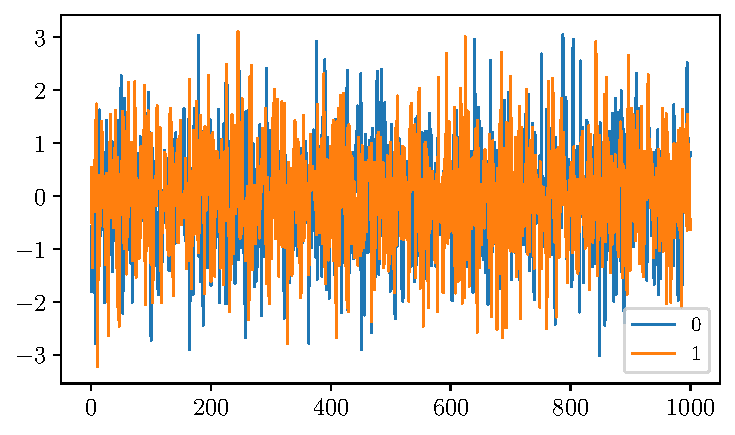
\includegraphics[width = 0.95\textwidth]{figures/rolldecay_example.pdf}\end{center}
\vspace{-0.7cm}
\caption{Roll decay time series}
\label{fig:rolldecay_example}
\end{figure}
The oscillating motion can be described by a spring-mass-damper system
as seen in Fig.\ref{fig:spring_mass_damper}.
\begin{figure}[H]
\begin{center}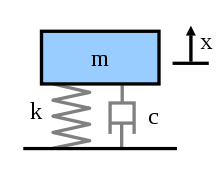
\includegraphics[width = 0.95\textwidth]{figures/spring_mass_damper.png}\end{center}
\vspace{-0.7cm}
\caption{Spring-mass-damper system}
\label{fig:spring_mass_damper}
\end{figure}
This system can me described as the following equation
\ref{eq:equation1}:
\begin{equation}
$E=m \dot c^2 $
\label{eq:equation1}
\end{equation}
\begin{equation}
A = \pi r^{2}
\label{eq:equation2}
\end{equation}
